\section{The Model - Part 1}
\subsection{Data and Results}



\begin{frame}
\frametitle{Data}

Since the paper examine the mita’s long-run impact on economic development by testing whether it affects living standards today, the data used was:

    \begin{itemize}

\item A list of districts subjected to the mita and matched to modern districts as detailed in the Supplemental Material.

    \end{itemize}
    For the measure of living standards two independent data sets are used:
    \begin{itemize}

\item 2001 Peruvian National Household Survey - collected by the National Institute of Statistics.\\[10pt]
\item Microcensus data set, obtained from the Ministry of Education, that records the heights of all 6- to 9-year- old school children in the region.

    \end{itemize}
  
\end{frame}



\begin{frame}
\frametitle{The basic model}



 \[ c_{idb} = \alpha + \gamma mita_{d} + X_{id}\beta + f(geographic location_{d}) + \delta_{b} + \epsilon_{idb}\]
 
 where :
 
 \begin{itemize}
 
 \item $c_{idb}$ is the outcome variable of interest for observation i in district d along segment b of the mita boundary.
 \item $mita_{d}$ is an indicator equal to 1 if district d contributed to the mita and equal to 0 otherwise.
 \item $ X_{id}$ is a vector of covariates that includes the mean area weighted elevation and slope for district d and demographic variables giving the number of infants, children, and adults in the household.
 \item $f(geographic location_{d})$ is the RD polynomial, which controls for smooth functions of geographic location.
 \item $\delta_{b}$ is a set of boundary segment fixed effects that denote which of four equal length segments of the boundary is the closest to the observations district capital.
 \end{itemize}
\end{frame}



\begin{frame}
\frametitle{Results}
\begin{center}
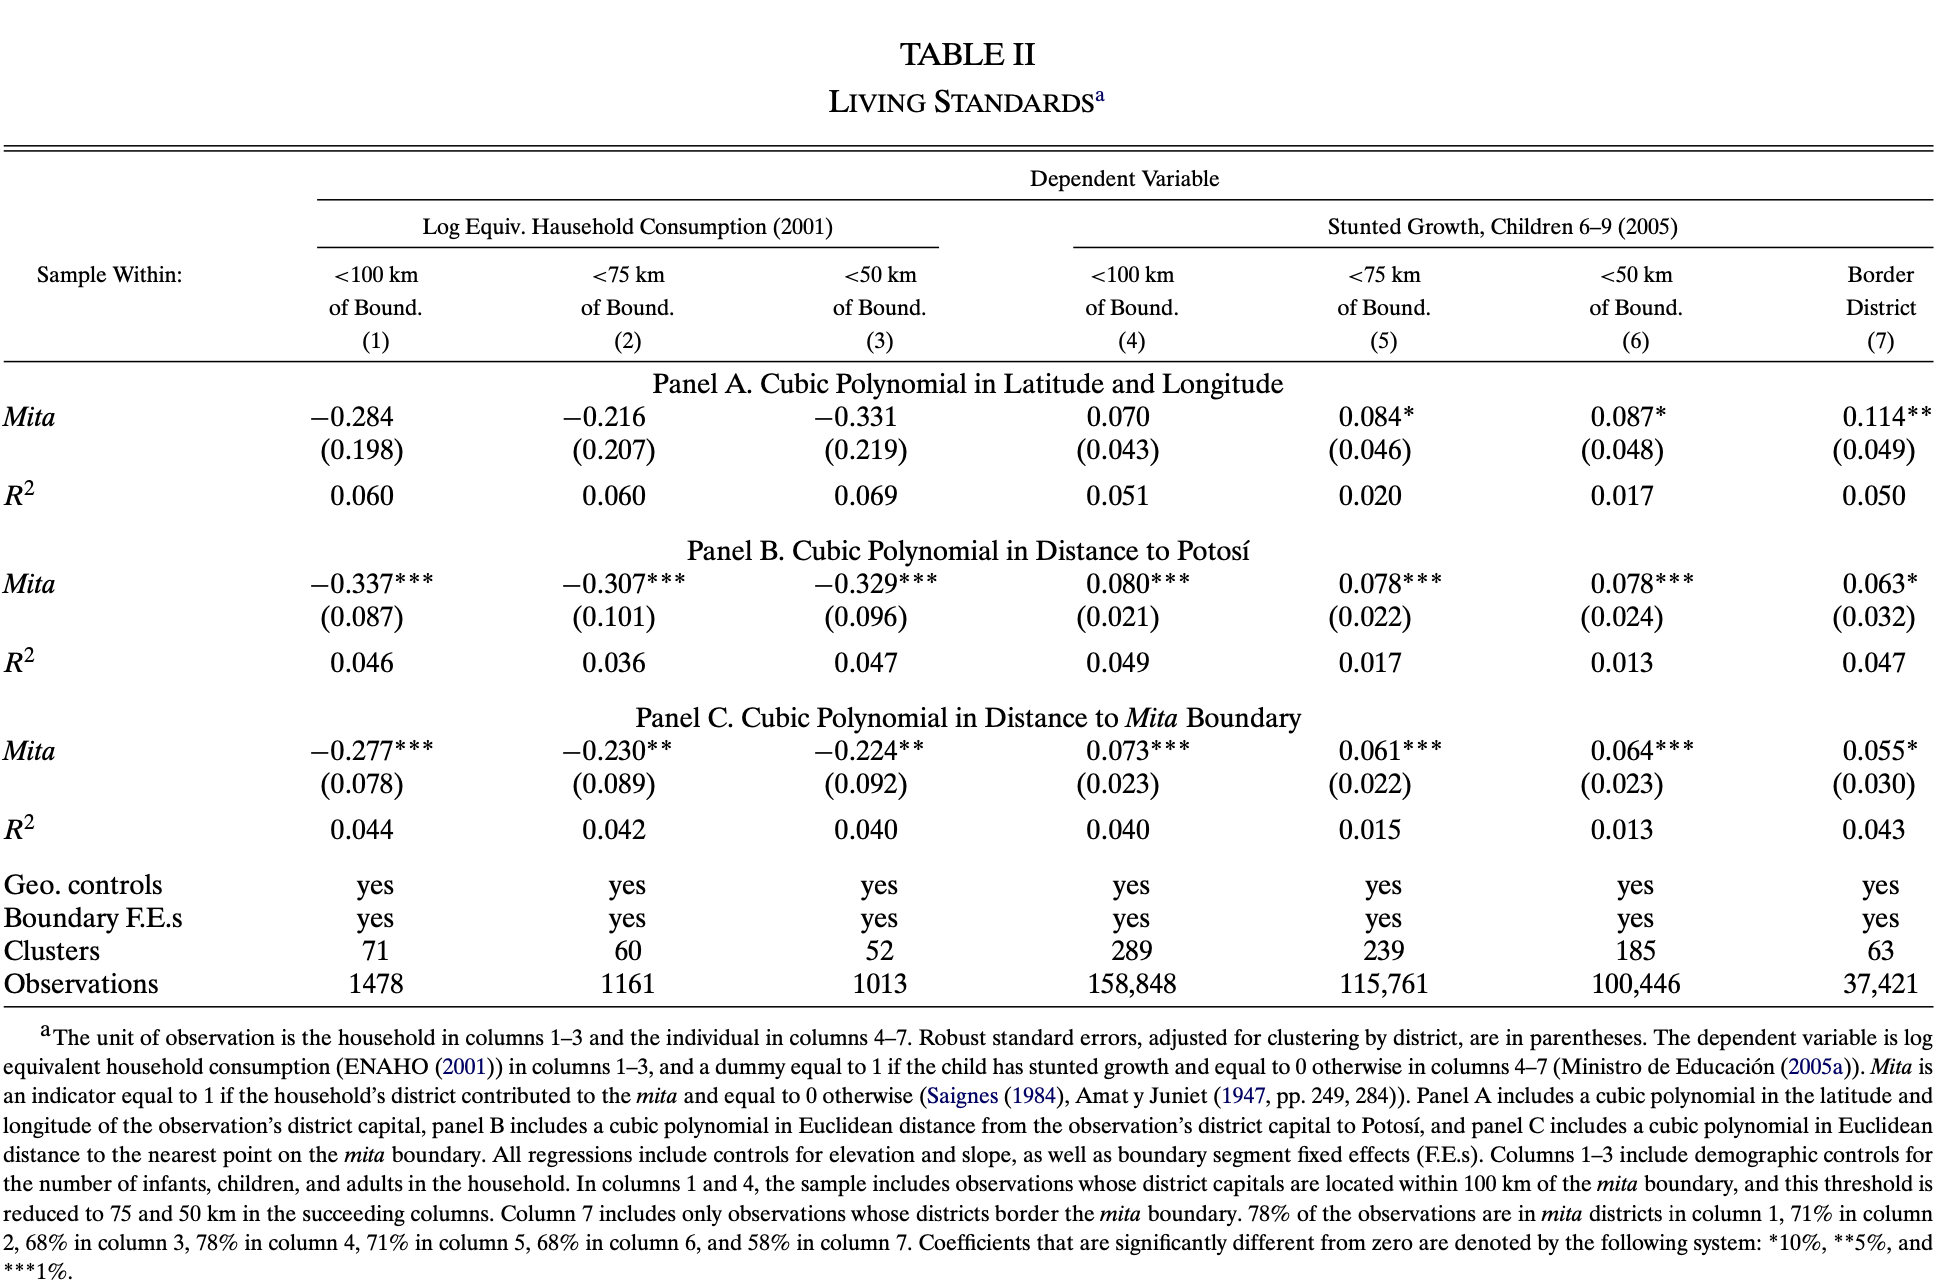
\includegraphics[width=1\textwidth] {Reg1.png}
\end{center}


\end{frame}



\begin{frame}
\frametitle{Results(Cont)}
\begin{itemize}
    \item Columns 1–3 of Table II estimate that a long-run mita effect lowers house- hold consumption in 2001 by around 25\% in subjected districts.\\[20pt]
    
    \item The mita coefficients are economically similar across the three specifications of the RD polynomial.\\[20pt]
    
    \item When using only observations in districts that border the mita boundary,point estimates of the mita effect on stunting range from 0.055 (s.e. = 0.030) to 0.114 (s.e. = 0.049) percentage points.
\end{itemize}

\end{frame}

\begin{frame}
\frametitle{Robustness tests}
\begin{center}
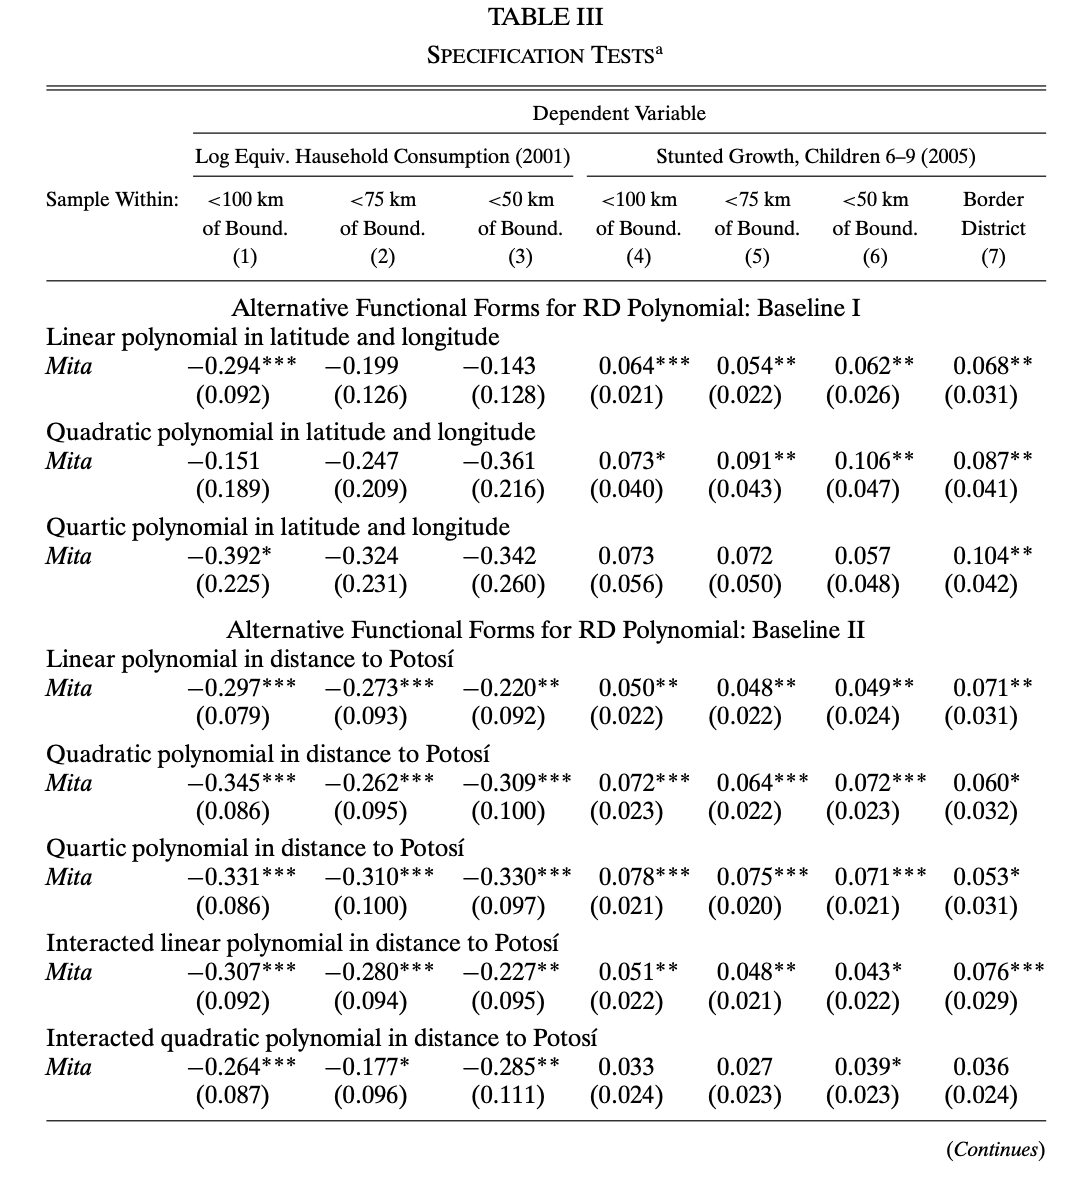
\includegraphics[width=.7\textwidth] {Perutabla3.png}
\end{center}
\end{frame}

\begin{frame}
\frametitle{Robustness tests}
\begin{center}
    

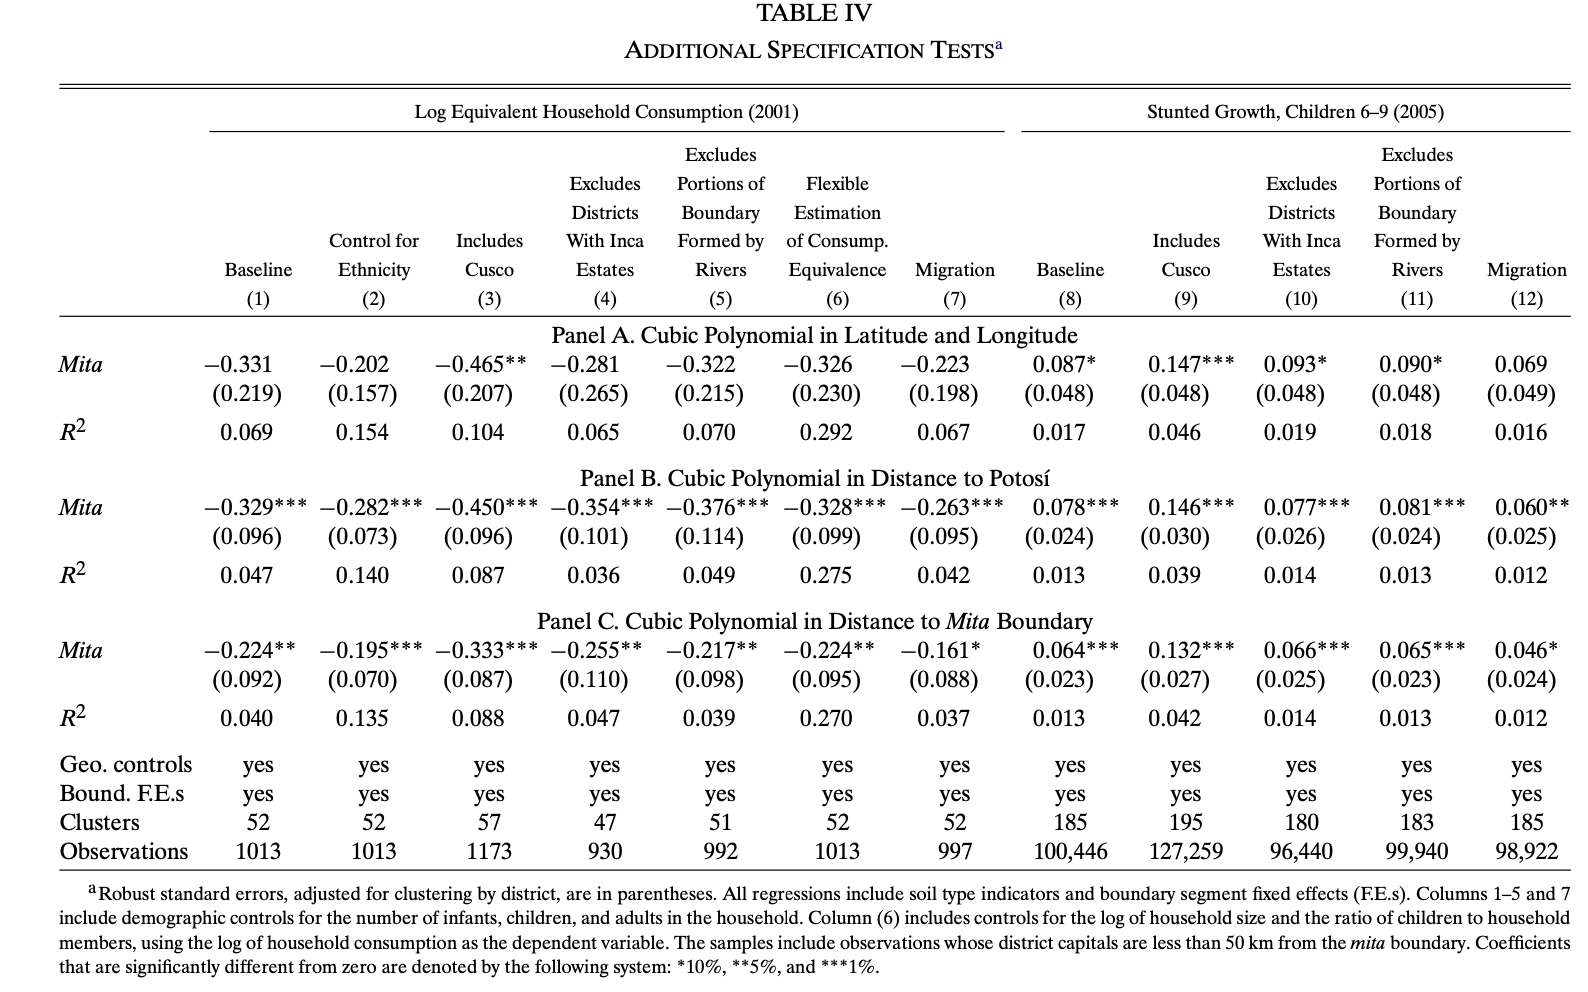
\includegraphics[width=1\textwidth] {Peru4.png}
\end{center}
\end{frame}
